\subsection{Decoupling of translational and rotational motion}\label{sec:DecouplingRigidBody}
The closed loop equations for a (free) three dimensional rigid body were given in \autoref{sec:CtrlApproachParticlesSingleBody}, \autoref{sec:CtrlApproachBodySingleBody} and \autoref{sec:CtrlApproachEnergySingleBody}.
The reduced equations for the planar case were given in \autoref{sec:CtrlPlanarRigidBody}.
For most applications we like to \textit{decouple} the translational and the rotational motion of the body.
%What this means and how it is achieved is discussed in this subsection.

Observing the closed loop equations one can see immediately that the coupling terms vanish if $\sc=\lc=\hc=\tuple{0}$, i.e.\ the the chosen body fixed point $\r$ coincides with the center of mass, damping and stiffness.
Then the rotational dynamics are identical to the closed loop given in \autoref{sec:CtrlExampleRigidBodyOrientation} (\autoref{sec:CtrlExampleRevoluteJoint} for the planar case), so are indeed decoupled/independent from the translational motion.

\paragraph{Translational dynamics.}
For the translational dynamics the situation is more difficult:
Introduce $\tuple{e} = \r-\rR$ as the components of the position error w.r.t.\ the inertial frame and $\rE = \RR^\top(\r-\rR)$ as the components w.r.t.\ the reference frame.
The translational dynamics for the different approaches and given transport map are equivalent to
\begin{subequations}\label{eq:RigidBodyPosErrorDyn}
\begin{align}
 &\text{particle-based:}&
 \mc\ddot{\tuple{e}} + \dc\dot{\tuple{e}} + \kc\tuple{e} &= \tuple{0}
\\
 &\text{body-based:}&
 \mc\rEdd + \dc\rEd + \kc\rE &= \tuple{0}
\\
 &\text{energy-based:}&
 \mc \big(\rEdd + \wedOp(\wR) \rEd \big) + \dc\rEd + \kc\rE &= \tuple{0}
 \label{eq:RigidBodyPosErrorDynApproach1}
% \\
%  &\text{approach 1 with \eqref{eq:RigidBodyAlternativeTransportMap}:}&
%  \mc\ddot{\tuple{e}} + \dc\dot{\tuple{e}} + \kc\tuple{e} &= \tuple{0}
\end{align}
\end{subequations}
% Obviously, for approach 1 with the transport map from \eqref{eq:RigidBodyAlternativeTransportMap} and approach 2, the error components $\tuple{e}$ w.r.t.\ the inertial frame obey linear dynamics.
% The same holds for approach 3 for the error components $\rE$ w.r.t.\ the reference frame.
% There is no transformation of the error coordinates to achieve this for approach 1 with the transport map from \eqref{eq:TransportMapRigidBody}.
% It is crucial to notice that all equations are indeed independent from the actual orientation $\R$ and angular velocity $\w$, but some do depend on their \textit{reference} $\RR$ and $\wR$.

\paragraph{Translational energy.}
For the rigid body we can split the total energy $\totalEnergyC = \totalEnergyC_{\r} + \totalEnergyC_{\R}$ into a part associated with the position $\totalEnergyC_{\r}$ and one associated with the orientation $\totalEnergyC_{\R}$.
The rotational energies for the corresponding approaches coincide with the ones given in \autoref{sec:CtrlExampleRigidBodyOrientation} (\autoref{sec:CtrlExampleRevoluteJoint} for the planar case).
The translational energies and their derivatives are
\begin{subequations}
\begin{align}
 &\text{particle-based:}&
 \totalEnergyC_{\r} &= \tfrac{1}{2} \kc \norm{\tuple{e}}^2 + \tfrac{1}{2} \mc \norm{\dot{\tuple{e}}}^2,&
 \dot{\totalEnergyC}_{\r} &= -\dc\norm{\dot{\tuple{e}}}^2
\\
 &\text{body-based:}&
 \totalEnergyC_{\r} &= \tfrac{1}{2} \kc \norm{\rE}^2 + \tfrac{1}{2} \mc \norm{\rEd}^2,&
 \dot{\totalEnergyC}_{\r} &= -\dc\norm{\rEd}^2 
\\
 &\text{energy-based:}&
 \totalEnergyC_{\r} &= \tfrac{1}{2} \kc \norm{\rE}^2 + \tfrac{1}{2} \mc \norm{\rEd}^2,&
 \dot{\totalEnergyC}_{\r} &= -\dc\norm{\rEd}^2 
%  &\text{approach 1 with \eqref{eq:RigidBodyAlternativeTransportMap}:}&
%  \totalEnergyC_{\r} &= \tfrac{1}{2} \kc \norm{\tuple{e}}^2 + \tfrac{1}{2} \mc \norm{\dot{\tuple{e}}}^2,&
%  \dot{\totalEnergyC}_{\r} &= -\dc\norm{\dot{\tuple{e}}}^2 
\end{align}
\end{subequations}
For their comparison note that
\begin{align}
 \norm{\tuple{e}} = \norm{\rE},
\qquad
 \norm{\dot{\tuple{e}}} = \norm{\rEd + \wedOp(\wR) \rE}.
\end{align}

The crucial observation is that for all approaches the translational dynamics and energy are indeed independent of the actual orientation $\R$ and its velocity $\w$, but for some approaches they depend on their \textit{reference} $\RR$ and $\wR$.
For a constant reference orientation $\RR = \const$ and consequently $\wR = \tuple{0}$ all four approaches are equivalent.
Furthermore it is worth noting that the error dynamics as well as the energies are invariant to the reference trajectory $t\mapsto\rR(t)$ for the position.

\paragraph{Simulation.}
The difference between these cases will be discussed on simulation results for the simpler, yet as illustrative, example of a planar rigid body:
The reference configuration is $\rxR(t) = \ryR(t) = 0$ and $\alpha_{\idxRef}(t) = \pi t$ which yields the constant reference velocity $\sysVelR(t) = [0,0,\pi]$.
The control parameters are set to $\mc=1$, $\dc=4$, $\kc=4$ (neglecting the units).
The roots of the characteristic polynomial of \eqref{eq:RigidBodyPosErrorDynApproach1} are $\lambda \approx \{-0.5 \pm 0.6\mathrm{i}, -3.5 \pm 3.7\mathrm{i} \}$, resulting from the control parameters as well as the constant angular velocity $\wzR=\pi$.
The characteristic polynomial for the other approaches is independent of the reference trajectory and has a quadruple root at $\lambda = -2$.

\autoref{fig:RBCtrlPosError} shows the simulation result for the initial conditions $\rx(0) = 0, \ry(0) = 1$, $\alpha(0) = 0$ and $\sysVel(0) = \tuple{0}$.
Observing from the inertial frame, top left of \autoref{fig:RBCtrlPosError}, for approach 2 the body follows a straight line to its reference position, whereas for the other approaches spiral around it.
Observing from the reference frame, top right of \autoref{fig:RBCtrlPosError}, for approach 3 the body follows a direct path, given the initial velocity.
The middle graph in \autoref{fig:RBCtrlPosError} shows the evolution of the translational energy $\totalEnergyC_{\r}$.
The difference in the initial values results from $\dot{\tuple{e}}(0) = \tuple{0}$, but $\rEd(0) \neq \tuple{0}$.
The bottom graph in \autoref{fig:RBCtrlPosError} shows the evolution of the euclidean distance $\norm{\tuple{e}} = \norm{\rE}$.
The rate of convergence for approach 2 and 3 are the same as could be expected from having the same characteristic polynomial.

Even though the energy based approach with the transport map from \eqref{eq:TimeDerivativeRigidBodxPotential} might be mathematically the most elegant solution, its simulation result is not intuitive.
Which approach is most desirable, depends given application.
For indoor robots (like the multicopters discussed in the next chapter) it is probably most desirable if it corrects its position error following a straight line in the inertial frame.

\begin{figure}[ht]
 \centering
 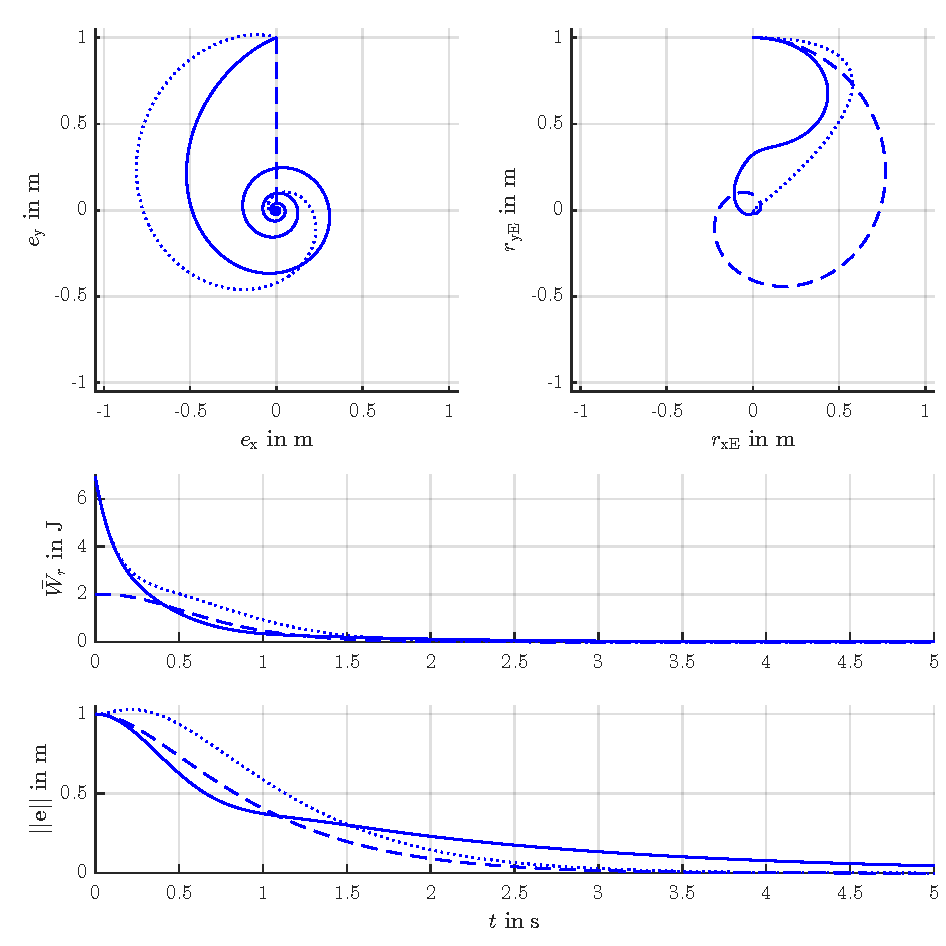
\includegraphics{PlanarRigidBody/RBCtrlPosError}
 \caption{Simulation result for the planar rigid body. The solid line: energy-based approach with $\sysTransportMap = \Ad{\bodyHomoCoord{}{}^{-1}\bodyHomoCoordR{}{}}$, dashed line: particle-based approach, dotted line: body-based approach.}
 \label{fig:RBCtrlPosError}
\end{figure}

% \paragraph{Approach 2}
% \begin{align*}
%  \mc (\vd + \wedOp(\w) \v - \RE^\top (\vRd + \wedOp(\wR)\vR) ) + \dc(\v - \RE^\top\vR) + \kc \R^\top(\r-\rR) &= \tuple{0}
% % \\
% %  \mc (\R^\top\rdd - \wedOp(\w)\R^\top \rd + \wedOp(\w) \R^\top \rd - \R^\top\RR (\RR^\top\rRdd - \wedOp(\wR)\RR^\top \rRd + \wedOp(\wR)\RR^\top\rRd) ) + \dc\R^\top(\rd - \rRd) + \kc \R^\top(\r-\rR) &= \tuple{0}
% \\
%  \Leftrightarrow\qquad
%  \mc\ddot{\tuple{e}} + \dc\dot{\tuple{e}} + \kc\tuple{e} &= \tuple{0}
% \end{align*}
% 
% 
% \paragraph{Approach 3}
% \begin{align*}
%  \mc \big(\vEd + \wedOp(\wE) \vE\big) + \dc\vE + \kc \R^\top(\r-\rR) &= \tuple{0}
% \\
%  \Leftrightarrow \qquad
%  \mc \big( \ddot{\tuple{e}} - 2\wedOp(\RR \wR) \dot{\tuple{e}} - \big(\wedOp(\RR \wRd) - \wedOp(\RR \wR)^2\big) \tuple{e} \big)\qquad&
% \\+ \dc\big(\dot{\tuple{e}} - \wedOp(\RR \wR) \tuple{e} \big) + \kc\tuple{e} &= \tuple{0}
% \\
%  \mc\rEdd + \dc\rEd + \kc\rE &= \tuple{0}
% \end{align*}
% 
% 
% \paragraph{Error coordinates}
% \begin{align}
%  \underbrace{\begin{bmatrix} \RE & \rE \\ \mat{0} & 1 \end{bmatrix}}_{\bodyHomoCoordE{}{}} 
%  &= \underbrace{\begin{bmatrix} \RR^\top \R & \RR^\top (\r - \rR) \\ \mat{0} & 1 \end{bmatrix}}_{\bodyHomoCoordR{}{}^{-1}\bodyHomoCoord{}{}},&
% %  &= \underbrace{\begin{bmatrix} \RR^\top & -\RR^\top \rR \\ \mat{0} & 1 \end{bmatrix}}_{\bodyHomoCoordR{}{}^{-1}} 
% %  \underbrace{\begin{bmatrix} \R & \r \\ \mat{0} & 1 \end{bmatrix}}_{\bodyHomoCoord{}{}}
%  \underbrace{\begin{bmatrix} \vE \\ \wE \end{bmatrix}}_{\bodyVelE{}{}} 
%  &= \underbrace{\begin{bmatrix} \v \\ \w \end{bmatrix}}_{\bodyVel{}{}} 
%  - \underbrace{\begin{bmatrix} \RE^\top & -\RE^\top \wedOp\rE \\ \mat{0} & \RE^\top \end{bmatrix}}_{\Ad{\bodyHomoCoordE{}{}^{-1}}} 
%  \underbrace{\begin{bmatrix} \vR \\ \wR \end{bmatrix}}_{\bodyVelR{}{}}.
% \end{align}
% 
% \begin{align*}
%  \vE &= \v - \R^\top \RR \vR + \R^\top \RR \wedOp(\RR^\top(\r-\rR)) \wR,
% \\
%  &= \R^\top \big(\dot{\tuple{e}} - \wedOp(\RR \wR) \tuple{e} \big),
% \\
%  &= \RE^\top \rEd,
% \\
%  \wE &= \w - \RE^\top \wR
% \end{align*}
% 
% 
% \paragraph{Approach 1}
% \begin{align*}
%  \mc \big(\vEd + \wedOp(\w) \vE\big) + \dc\vE + \kc \R^\top(\r-\rR) &= \tuple{0}
% \\
% %  \mc (\R^\top \rdd - \wedOp(\w)\R^\top \rd + \wedOp(\w)\R^\top (\rRd + \wedOp(\RR \wR) (\r-\rR))&
% % \\ -\R^\top (\rRdd + \wedOp(\RR \wRd) (\r-\rR) + \wedOp(\RR \wR) (\rd-\rRd))&
% % \\ + \wedOp(\w) (\R^\top\rd - \R^\top (\rRd + \wedOp(\RR \wR) (\r-\rR))))&
% % \\ + \dc(\R^\top\rd - \R^\top (\rRd + \wedOp(\RR \wR) (\r-\rR))) + \kc \R^\top(\r-\rR) &= \tuple{0}
% % \\
%  \Leftrightarrow\qquad 
%  \mc \big(\ddot{\tuple{e}} - \wedOp(\RR \wR) \dot{\tuple{e}} - \wedOp(\RR \wRd) \tuple{e} \big) + \dc(\dot{\tuple{e}} - \wedOp(\RR \wR) \tuple{e}) + \kc \tuple{e} &= \tuple{0}
% \\
%  \Leftrightarrow\qquad 
%  \mc \big(\rEdd + \wedOp(\wR) \rEd \big) + \dc\rEd + \kc\rE &= \tuple{0}
% \end{align*}
% 
% \paragraph{Approach 2}
% \begin{align*}
%  \mc (\vd + \wedOp(\w) \v - \RE^\top (\vRd + \wedOp(\wR)\vR) ) + \dc(\v - \RE^\top\vR) + \kc \R^\top(\r-\rR) &= \tuple{0}
% % \\
% %  \mc (\R^\top\rdd - \wedOp(\w)\R^\top \rd + \wedOp(\w) \R^\top \rd - \R^\top\RR (\RR^\top\rRdd - \wedOp(\wR)\RR^\top \rRd + \wedOp(\wR)\RR^\top\rRd) ) + \dc\R^\top(\rd - \rRd) + \kc \R^\top(\r-\rR) &= \tuple{0}
% \\
%  \Leftrightarrow\qquad
%  \mc\ddot{\tuple{e}} + \dc\dot{\tuple{e}} + \kc\tuple{e} &= \tuple{0}
% \end{align*}
% 
% 
% \paragraph{Approach 3}
% \begin{align*}
%  \mc \big(\vEd + \wedOp(\wE) \vE\big) + \dc\vE + \kc \R^\top(\r-\rR) &= \tuple{0}
% \\
%  \Leftrightarrow \qquad
%  \mc \big( \ddot{\tuple{e}} - 2\wedOp(\RR \wR) \dot{\tuple{e}} - \big(\wedOp(\RR \wRd) - \wedOp(\RR \wR)^2\big) \tuple{e} \big)\qquad&
% \\+ \dc\big(\dot{\tuple{e}} - \wedOp(\RR \wR) \tuple{e} \big) + \kc\tuple{e} &= \tuple{0}
% \\
%  \mc\rEdd + \dc\rEd + \kc\rE &= \tuple{0}
% \end{align*}
